\documentclass[11pt,]{article}
\usepackage[left=1in,top=1in,right=1in,bottom=1in]{geometry}
\newcommand*{\authorfont}{\fontfamily{phv}\selectfont}
\usepackage[]{mathpazo}


  \usepackage[T1]{fontenc}
  \usepackage[utf8]{inputenc}



\usepackage{abstract}
\renewcommand{\abstractname}{}    % clear the title
\renewcommand{\absnamepos}{empty} % originally center

\renewenvironment{abstract}
 {{%
    \setlength{\leftmargin}{0mm}
    \setlength{\rightmargin}{\leftmargin}%
  }%
  \relax}
 {\endlist}

\makeatletter
\def\@maketitle{%
  \newpage
%  \null
%  \vskip 2em%
%  \begin{center}%
  \let \footnote \thanks
    {\fontsize{18}{20}\selectfont\raggedright  \setlength{\parindent}{0pt} \@title \par}%
}
%\fi
\makeatother




\setcounter{secnumdepth}{0}

\usepackage{color}
\usepackage{fancyvrb}
\newcommand{\VerbBar}{|}
\newcommand{\VERB}{\Verb[commandchars=\\\{\}]}
\DefineVerbatimEnvironment{Highlighting}{Verbatim}{commandchars=\\\{\}}
% Add ',fontsize=\small' for more characters per line
\usepackage{framed}
\definecolor{shadecolor}{RGB}{248,248,248}
\newenvironment{Shaded}{\begin{snugshade}}{\end{snugshade}}
\newcommand{\KeywordTok}[1]{\textcolor[rgb]{0.13,0.29,0.53}{\textbf{#1}}}
\newcommand{\DataTypeTok}[1]{\textcolor[rgb]{0.13,0.29,0.53}{#1}}
\newcommand{\DecValTok}[1]{\textcolor[rgb]{0.00,0.00,0.81}{#1}}
\newcommand{\BaseNTok}[1]{\textcolor[rgb]{0.00,0.00,0.81}{#1}}
\newcommand{\FloatTok}[1]{\textcolor[rgb]{0.00,0.00,0.81}{#1}}
\newcommand{\ConstantTok}[1]{\textcolor[rgb]{0.00,0.00,0.00}{#1}}
\newcommand{\CharTok}[1]{\textcolor[rgb]{0.31,0.60,0.02}{#1}}
\newcommand{\SpecialCharTok}[1]{\textcolor[rgb]{0.00,0.00,0.00}{#1}}
\newcommand{\StringTok}[1]{\textcolor[rgb]{0.31,0.60,0.02}{#1}}
\newcommand{\VerbatimStringTok}[1]{\textcolor[rgb]{0.31,0.60,0.02}{#1}}
\newcommand{\SpecialStringTok}[1]{\textcolor[rgb]{0.31,0.60,0.02}{#1}}
\newcommand{\ImportTok}[1]{#1}
\newcommand{\CommentTok}[1]{\textcolor[rgb]{0.56,0.35,0.01}{\textit{#1}}}
\newcommand{\DocumentationTok}[1]{\textcolor[rgb]{0.56,0.35,0.01}{\textbf{\textit{#1}}}}
\newcommand{\AnnotationTok}[1]{\textcolor[rgb]{0.56,0.35,0.01}{\textbf{\textit{#1}}}}
\newcommand{\CommentVarTok}[1]{\textcolor[rgb]{0.56,0.35,0.01}{\textbf{\textit{#1}}}}
\newcommand{\OtherTok}[1]{\textcolor[rgb]{0.56,0.35,0.01}{#1}}
\newcommand{\FunctionTok}[1]{\textcolor[rgb]{0.00,0.00,0.00}{#1}}
\newcommand{\VariableTok}[1]{\textcolor[rgb]{0.00,0.00,0.00}{#1}}
\newcommand{\ControlFlowTok}[1]{\textcolor[rgb]{0.13,0.29,0.53}{\textbf{#1}}}
\newcommand{\OperatorTok}[1]{\textcolor[rgb]{0.81,0.36,0.00}{\textbf{#1}}}
\newcommand{\BuiltInTok}[1]{#1}
\newcommand{\ExtensionTok}[1]{#1}
\newcommand{\PreprocessorTok}[1]{\textcolor[rgb]{0.56,0.35,0.01}{\textit{#1}}}
\newcommand{\AttributeTok}[1]{\textcolor[rgb]{0.77,0.63,0.00}{#1}}
\newcommand{\RegionMarkerTok}[1]{#1}
\newcommand{\InformationTok}[1]{\textcolor[rgb]{0.56,0.35,0.01}{\textbf{\textit{#1}}}}
\newcommand{\WarningTok}[1]{\textcolor[rgb]{0.56,0.35,0.01}{\textbf{\textit{#1}}}}
\newcommand{\AlertTok}[1]{\textcolor[rgb]{0.94,0.16,0.16}{#1}}
\newcommand{\ErrorTok}[1]{\textcolor[rgb]{0.64,0.00,0.00}{\textbf{#1}}}
\newcommand{\NormalTok}[1]{#1}

\usepackage{graphicx,grffile}
\makeatletter
\def\maxwidth{\ifdim\Gin@nat@width>\linewidth\linewidth\else\Gin@nat@width\fi}
\def\maxheight{\ifdim\Gin@nat@height>\textheight\textheight\else\Gin@nat@height\fi}
\makeatother
% Scale images if necessary, so that they will not overflow the page
% margins by default, and it is still possible to overwrite the defaults
% using explicit options in \includegraphics[width, height, ...]{}
\setkeys{Gin}{width=\maxwidth,height=\maxheight,keepaspectratio}

\title{S13 - Clasificacion no supervizada  }



\author{\Large Juan Carlos Martinez-Ovando\vspace{0.05in} \newline\normalsize\emph{}  }


\date{}

\usepackage{titlesec}

\titleformat*{\section}{\normalsize\bfseries}
\titleformat*{\subsection}{\normalsize\itshape}
\titleformat*{\subsubsection}{\normalsize\itshape}
\titleformat*{\paragraph}{\normalsize\itshape}
\titleformat*{\subparagraph}{\normalsize\itshape}


\usepackage{natbib}
\bibliographystyle{plainnat}
\usepackage[strings]{underscore} % protect underscores in most circumstances



\newtheorem{hypothesis}{Hypothesis}
\usepackage{setspace}

\makeatletter
\@ifpackageloaded{hyperref}{}{%
\ifxetex
  \PassOptionsToPackage{hyphens}{url}\usepackage[setpagesize=false, % page size defined by xetex
              unicode=false, % unicode breaks when used with xetex
              xetex]{hyperref}
\else
  \PassOptionsToPackage{hyphens}{url}\usepackage[unicode=true]{hyperref}
\fi
}

\@ifpackageloaded{color}{
    \PassOptionsToPackage{usenames,dvipsnames}{color}
}{%
    \usepackage[usenames,dvipsnames]{color}
}
\makeatother
\hypersetup{breaklinks=true,
            bookmarks=true,
            pdfauthor={Juan Carlos Martinez-Ovando ()},
             pdfkeywords = {Probabilistic graphical models, latent variables, extended likelihood,
distace-based clustering.},  
            pdftitle={S13 - Clasificacion no supervizada},
            colorlinks=true,
            citecolor=blue,
            urlcolor=blue,
            linkcolor=magenta,
            pdfborder={0 0 0}}
\urlstyle{same}  % don't use monospace font for urls

% set default figure placement to htbp
\makeatletter
\def\fps@figure{htbp}
\makeatother



% add tightlist ----------
\providecommand{\tightlist}{%
\setlength{\itemsep}{0pt}\setlength{\parskip}{0pt}}

\begin{document}
	
% \pagenumbering{arabic}% resets `page` counter to 1 
%
% \maketitle

{% \usefont{T1}{pnc}{m}{n}
\setlength{\parindent}{0pt}
\thispagestyle{plain}
{\fontsize{18}{20}\selectfont\raggedright 
\maketitle  % title \par  

}

{
   \vskip 13.5pt\relax \normalsize\fontsize{11}{12} 
\textbf{\authorfont Juan Carlos Martinez-Ovando} \hskip 15pt \emph{\small }   

}

}








\begin{abstract}

    \hbox{\vrule height .2pt width 39.14pc}

    \vskip 8.5pt % \small 

\noindent En la sesion de hoy revisaremos comparativamente dos metodos de
clasificacion no supervisada (clustering) de datos escalares
\(d\)-dimensionales. Revisaremos en detalle dos algoritmos para su
implementacion.


\vskip 8.5pt \noindent \emph{Keywords}: Probabilistic graphical models, latent variables, extended likelihood,
distace-based clustering. \par

    \hbox{\vrule height .2pt width 39.14pc}



\end{abstract}


\vskip 6.5pt


\noindent \doublespacing \section{Simulacion de datos}\label{simulacion-de-datos}

Generamos una muestra de \(n\) variables escalaras de una mezcla de
\(K\) distribuciones gausianas \(d\) dimensionales. En el siguiente
script, \(k\) es el numero de grupos o clases, \(\mu\) es una matriz de
dimension \(k \times d\) con vectores de medias para cada grupo, y
\(\Sigma\) es un arreglo de dimension \(K \times d \times d\) de
matrices de covarianza.

\begin{Shaded}
\begin{Highlighting}[]
\NormalTok{rmixgaussian <-}\StringTok{ }\ControlFlowTok{function}\NormalTok{(n, k, mu, sig) \{}
  \ControlFlowTok{if}\NormalTok{(}\OperatorTok{!}\KeywordTok{require}\NormalTok{(}\StringTok{'MASS'}\NormalTok{))\{}\KeywordTok{install.packages}\NormalTok{(}\StringTok{"MASS"}\NormalTok{)\} }
  \KeywordTok{library}\NormalTok{(}\StringTok{"MASS"}\NormalTok{)}

\NormalTok{  d <-}\StringTok{ }\KeywordTok{length}\NormalTok{(mu[}\DecValTok{1}\NormalTok{,])}
\NormalTok{  result <-}\StringTok{ }\KeywordTok{matrix}\NormalTok{(}\KeywordTok{rep}\NormalTok{(}\OtherTok{NA}\NormalTok{,n}\OperatorTok{*}\NormalTok{d), }\DataTypeTok{ncol=}\NormalTok{d)}
  \KeywordTok{colnames}\NormalTok{(result) <-}\StringTok{ }\KeywordTok{paste0}\NormalTok{(}\StringTok{"X"}\NormalTok{,}\DecValTok{1}\OperatorTok{:}\NormalTok{d)}
  
  \ControlFlowTok{for}\NormalTok{(i }\ControlFlowTok{in} \DecValTok{1}\OperatorTok{:}\NormalTok{n) \{}
\NormalTok{    result[i,] <-}\StringTok{ }\KeywordTok{mvrnorm}\NormalTok{(}\DecValTok{1}\NormalTok{, }\DataTypeTok{mu =}\NormalTok{ mu[k[i],], }\DataTypeTok{Sigma=}\NormalTok{sig[,,k[i]])}
\NormalTok{  \}}
  \KeywordTok{return}\NormalTok{(result)}
\NormalTok{\}}
\end{Highlighting}
\end{Shaded}

Los datos simulados son:

\begin{Shaded}
\begin{Highlighting}[]
\KeywordTok{set.seed}\NormalTok{(}\DecValTok{123}\NormalTok{)}

\NormalTok{n <-}\StringTok{ }\DecValTok{360}

\NormalTok{mu <-}\StringTok{ }\KeywordTok{matrix}\NormalTok{(}\KeywordTok{c}\NormalTok{(}\FloatTok{14.0}\NormalTok{,}\FloatTok{4.0}\NormalTok{,}
               \FloatTok{15.0}\NormalTok{,}\FloatTok{5.0}\NormalTok{,}
               \FloatTok{16.5}\NormalTok{,}\FloatTok{5.0}\NormalTok{), }\DataTypeTok{ncol=}\DecValTok{2}\NormalTok{, }\DataTypeTok{byrow=}\NormalTok{T)}

\NormalTok{sigs <-}\StringTok{ }\KeywordTok{array}\NormalTok{(}\KeywordTok{rep}\NormalTok{(}\OtherTok{NA}\NormalTok{,}\DecValTok{2}\OperatorTok{*}\DecValTok{2}\OperatorTok{*}\DecValTok{3}\NormalTok{), }\KeywordTok{c}\NormalTok{(}\DecValTok{2}\NormalTok{,}\DecValTok{2}\NormalTok{,}\DecValTok{3}\NormalTok{))}

\NormalTok{sigs[,,}\DecValTok{1}\NormalTok{] <-}\StringTok{ }\KeywordTok{matrix}\NormalTok{(}\KeywordTok{c}\NormalTok{(.}\DecValTok{25}\NormalTok{, .}\DecValTok{21}\NormalTok{, .}\DecValTok{21}\NormalTok{,.}\DecValTok{25}\NormalTok{), }\DataTypeTok{nrow=}\DecValTok{2}\NormalTok{, }\DataTypeTok{byrow=}\OtherTok{TRUE}\NormalTok{)}
\NormalTok{sigs[,,}\DecValTok{2}\NormalTok{] <-}\StringTok{ }\KeywordTok{matrix}\NormalTok{(}\KeywordTok{c}\NormalTok{(.}\DecValTok{25}\NormalTok{,}\OperatorTok{-}\NormalTok{.}\DecValTok{21}\NormalTok{,}\OperatorTok{-}\NormalTok{.}\DecValTok{21}\NormalTok{,.}\DecValTok{25}\NormalTok{), }\DataTypeTok{nrow=}\DecValTok{2}\NormalTok{, }\DataTypeTok{byrow=}\OtherTok{TRUE}\NormalTok{)}
\NormalTok{sigs[,,}\DecValTok{3}\NormalTok{] <-}\StringTok{ }\KeywordTok{matrix}\NormalTok{(}\KeywordTok{c}\NormalTok{(.}\DecValTok{25}\NormalTok{, .}\DecValTok{21}\NormalTok{, .}\DecValTok{21}\NormalTok{,.}\DecValTok{25}\NormalTok{), }\DataTypeTok{nrow=}\DecValTok{2}\NormalTok{, }\DataTypeTok{byrow=}\OtherTok{TRUE}\NormalTok{)}

\NormalTok{pi <-}\StringTok{ }\KeywordTok{c}\NormalTok{(.}\DecValTok{2}\NormalTok{,.}\DecValTok{5}\NormalTok{,.}\DecValTok{3}\NormalTok{)}

\NormalTok{classes <-}\StringTok{ }\KeywordTok{sample}\NormalTok{(}\DecValTok{1}\OperatorTok{:}\DecValTok{3}\NormalTok{, n, }\DataTypeTok{replace=}\OtherTok{TRUE}\NormalTok{, }\DataTypeTok{prob=}\NormalTok{pi)}

\NormalTok{data <-}\StringTok{ }\KeywordTok{rmixgaussian}\NormalTok{(n, classes, mu, sigs)}
\end{Highlighting}
\end{Shaded}

\begin{verbatim}
## Loading required package: MASS
\end{verbatim}

\subsubsection{Datos}\label{datos}

Pretendiendo no conocer con anticipacion como los datos son generado o,
inclusive, si estos estan segmentados, su representacion grafica seria
de la siguiente forma.

\begin{Shaded}
\begin{Highlighting}[]
\KeywordTok{plot}\NormalTok{(data, }\DataTypeTok{col=}\StringTok{"black"}\NormalTok{, }\DataTypeTok{xlab=}\StringTok{"X1"}\NormalTok{, }\DataTypeTok{ylab=}\StringTok{"X2"}\NormalTok{, }\DataTypeTok{pch=}\DecValTok{19}\NormalTok{)}
\end{Highlighting}
\end{Shaded}

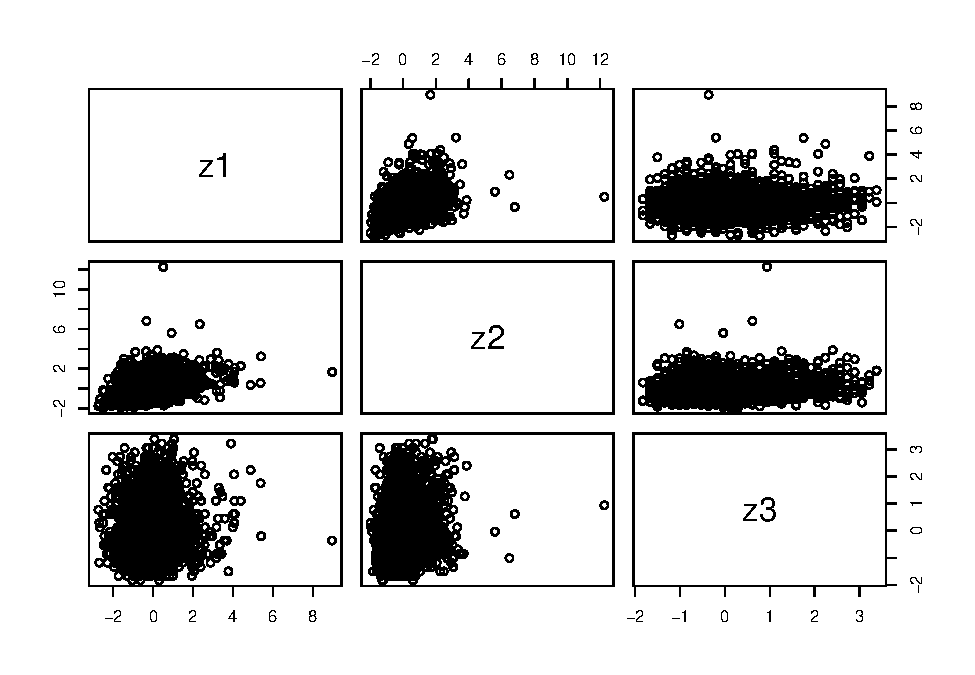
\includegraphics{est46114_s13_unsupervisedclassification_files/figure-latex/unnamed-chunk-1-1.pdf}

Aunque sabiendo el mecanismo que genero los datos, la representacion
grafica de los mismos deberia de ser de la siguiente forma.

\begin{Shaded}
\begin{Highlighting}[]
\KeywordTok{plot}\NormalTok{(data, }\DataTypeTok{col=}\KeywordTok{c}\NormalTok{(}\StringTok{"red"}\NormalTok{,}\StringTok{"green"}\NormalTok{,}\StringTok{"blue"}\NormalTok{)[classes], }\DataTypeTok{xlab=}\StringTok{"X1"}\NormalTok{, }\DataTypeTok{ylab=}\StringTok{"X2"}\NormalTok{, }\DataTypeTok{pch=}\DecValTok{19}\NormalTok{)}
\end{Highlighting}
\end{Shaded}

\includegraphics{est46114_s13_unsupervisedclassification_files/figure-latex/unnamed-chunk-2-1.pdf}

Los metodos que revisaremos hoy tiene como proposito revelar estructuras
de agrupamiento en datos que no conocemos con antelacion. La primera es
basada en la nocion geometrica de distancia (\textbf{K-means}) y la
segunda basada en argumentos de mezclas de modelos (\textbf{mixture of
gaussian}).

Notaran que la segunda, en el contexto controlado de esta nota la opcion
\textbf{mixture of gaussian} puede parecer mas adecuada. Sin embargo,
ambos modelos sirven al mismo proposito. En clase comentaremos que
aspectos son relevantes para uno u otro.

\section{K-means}\label{k-means}

El algoritmo de clasificacion \textbf{K-mean} funciona como un algoritmo
iterativo de asignacion de clases basado en un conjunto de datos y una
distancia (tipicamente la distancia euclidiana). El algoritmo funciona
sobre un conjunto de datos \(x=x(x_i)^{n}_{i=1}\) \(d\)-dimensionales, y
un numero fijo de clases o grupos \(K\).

Cada grupo \(k\) es caracterizado por un centroide, \(m_k\) definido
itertivamente como la media aritmetica de los datos que componen el
grupo \(k\), siendo el grupo \(k\) definido como el conjunto de datos
que minimiza la suma de cuadrados de las distancias de los datos a los
centroides correspondientes.

El algoritmo se puede expresar como un problema de decision empleando la
funcion objetivo \[
J(x,K,\mu)=\sum_{i=1}^{n}\sum_{k=1}^{K}r_{ik} d(x_i,\mu_k),
\] donde

\begin{itemize}
\item
  \(r_i=(r_{i1,\ldots,r_{iK}})\) es la variable indicadora
  \(K\)-dimensional para la que solo una entrada es igual a 1 (la
  entrada correspondiente al grupo en el que la observacion \(i\) es
  asignada a la clase \(k\))
\item
  \(\mu=(\mu_i)_{i=1}^{K}\) es la coleccion de centroides de las \(K\)
  clases
\item
  \(d(x_i,\mu_k)\) es la distancia (euclidiana) del punto \(x_i\) al
  centroide \(\mu_k\).
\end{itemize}

\subsection{Asignacion}\label{asignacion}

La asignacion en este modelo consiste en minimizar la funcion \(J(x,K)\)
para \(r=(r_{i})_{i=1}^{n}\), dado los centroides \((\mu_k)_{k=1}^{K}\).
Y con base en las asignaciones \(r\) minimizar \(J(x,K,\mu)\) con
respecto a \(\mu\).

\subsubsection{Algoritmo}\label{algoritmo}

El algoritmo de este procedimiento se muestra a continuacion:

\begin{Shaded}
\begin{Highlighting}[]
\NormalTok{k.means <-}\StringTok{ }\ControlFlowTok{function}\NormalTok{(dataset, K, }\DataTypeTok{max_iter=}\DecValTok{100}\NormalTok{) \{}
  
\NormalTok{  get_classes <-}\StringTok{ }\ControlFlowTok{function}\NormalTok{(rnk)\{}
    \KeywordTok{apply}\NormalTok{(rnk,}\DecValTok{1}\NormalTok{,}\ControlFlowTok{function}\NormalTok{(row) }\KeywordTok{which.max}\NormalTok{(row))}
\NormalTok{    \}}
  
\NormalTok{  d <-}\StringTok{ }\KeywordTok{ncol}\NormalTok{(dataset)}
\NormalTok{  N <-}\StringTok{ }\KeywordTok{nrow}\NormalTok{(dataset)}
\NormalTok{  ranges <-}\StringTok{ }\KeywordTok{sapply}\NormalTok{(}\DecValTok{1}\OperatorTok{:}\NormalTok{d, }\ControlFlowTok{function}\NormalTok{ (i) }\KeywordTok{range}\NormalTok{(dataset[,i]))}
  
  \CommentTok{# K centroided iniciales}
\NormalTok{  mu <-}\StringTok{ }\KeywordTok{t}\NormalTok{(}\KeywordTok{replicate}\NormalTok{(K,}\KeywordTok{sapply}\NormalTok{(}\DecValTok{1}\OperatorTok{:}\NormalTok{d, }
                             \ControlFlowTok{function}\NormalTok{(i) }\KeywordTok{runif}\NormalTok{(}\DecValTok{1}\NormalTok{,ranges[}\DecValTok{1}\NormalTok{,i], ranges[}\DecValTok{2}\NormalTok{,i]))))}
  
\NormalTok{  rnk <-}\StringTok{ }\KeywordTok{matrix}\NormalTok{(}\KeywordTok{rep}\NormalTok{(}\DecValTok{0}\NormalTok{,K}\OperatorTok{*}\NormalTok{n), }\DataTypeTok{ncol=}\NormalTok{K)}
\NormalTok{  old_classes <-}\StringTok{ }\KeywordTok{get_classes}\NormalTok{(rnk)}
  
  \ControlFlowTok{for}\NormalTok{(it }\ControlFlowTok{in} \DecValTok{1}\OperatorTok{:}\NormalTok{max_iter) \{}
    \ControlFlowTok{for}\NormalTok{(n }\ControlFlowTok{in} \DecValTok{1}\OperatorTok{:}\NormalTok{N) \{}
\NormalTok{      distances <-}\StringTok{ }\KeywordTok{sapply}\NormalTok{(}\DecValTok{1}\OperatorTok{:}\NormalTok{K, }\ControlFlowTok{function}\NormalTok{(k) }
        \KeywordTok{norm}\NormalTok{(}\KeywordTok{as.matrix}\NormalTok{(dataset[n,]}\OperatorTok{-}\NormalTok{mu[k,]),}\StringTok{"F"}\NormalTok{))}
\NormalTok{      rnk[n,]   <-}\StringTok{ }\KeywordTok{rep}\NormalTok{(}\DecValTok{0}\NormalTok{,K)}
\NormalTok{      rnk[n,}\KeywordTok{which.min}\NormalTok{(distances)] <-}\StringTok{ }\DecValTok{1}
\NormalTok{    \}}
    
\NormalTok{    classes <-}\StringTok{ }\KeywordTok{get_classes}\NormalTok{(rnk)}
    \ControlFlowTok{if}\NormalTok{ (}\KeywordTok{all}\NormalTok{(old_classes }\OperatorTok{==}\StringTok{ }\NormalTok{classes))}
      \ControlFlowTok{break}
    \ControlFlowTok{else} 
\NormalTok{      old_classes <-}\StringTok{ }\NormalTok{classes}
    
    \ControlFlowTok{for}\NormalTok{(k }\ControlFlowTok{in} \DecValTok{1}\OperatorTok{:}\NormalTok{K) \{}
\NormalTok{      mu[k,]  <-}\StringTok{ }\NormalTok{rnk[,k] }\OperatorTok\StringTok{ }\NormalTok{dataset }\OperatorTok{/}\StringTok{ }\KeywordTok{sum}\NormalTok{(rnk[,k])}
\NormalTok{    \}}
\NormalTok{  \}}
\NormalTok{  output <-}\StringTok{ }\KeywordTok{list}\NormalTok{(}\DataTypeTok{mu=}\NormalTok{mu, }\DataTypeTok{pred=}\NormalTok{classes)}
  \KeywordTok{return}\NormalTok{(output)}
\NormalTok{\}}
\end{Highlighting}
\end{Shaded}

\begin{Shaded}
\begin{Highlighting}[]
\KeywordTok{set.seed}\NormalTok{(}\DecValTok{1231}\NormalTok{)}
\NormalTok{result <-}\StringTok{ }\KeywordTok{k.means}\NormalTok{(data,}\DecValTok{2}\NormalTok{)}

\KeywordTok{plot}\NormalTok{(data, }
     \DataTypeTok{col=}\KeywordTok{c}\NormalTok{(}\StringTok{"red"}\NormalTok{,}\StringTok{"green"}\NormalTok{,}\StringTok{"blue"}\NormalTok{)[result}\OperatorTok{$}\NormalTok{pred], }
     \DataTypeTok{xlab=}\StringTok{"X1"}\NormalTok{, }\DataTypeTok{ylab=}\StringTok{"X2"}\NormalTok{, }\DataTypeTok{pch=}\DecValTok{19}\NormalTok{)}
\KeywordTok{points}\NormalTok{(result}\OperatorTok{$}\NormalTok{mu, }\DataTypeTok{pch=}\DecValTok{3}\NormalTok{, }\DataTypeTok{lwd=}\DecValTok{4}\NormalTok{)}
\end{Highlighting}
\end{Shaded}

\includegraphics{est46114_s13_unsupervisedclassification_files/figure-latex/kmeans_2-1.pdf}

\begin{Shaded}
\begin{Highlighting}[]
\KeywordTok{set.seed}\NormalTok{(}\DecValTok{1231}\NormalTok{)}
\NormalTok{result <-}\StringTok{ }\KeywordTok{k.means}\NormalTok{(data,}\DecValTok{3}\NormalTok{)}

\KeywordTok{plot}\NormalTok{(data, }
     \DataTypeTok{col=}\KeywordTok{c}\NormalTok{(}\StringTok{"red"}\NormalTok{,}\StringTok{"green"}\NormalTok{,}\StringTok{"blue"}\NormalTok{)[result}\OperatorTok{$}\NormalTok{pred], }
     \DataTypeTok{xlab=}\StringTok{"X1"}\NormalTok{, }\DataTypeTok{ylab=}\StringTok{"X2"}\NormalTok{, }\DataTypeTok{pch=}\DecValTok{19}\NormalTok{)}
\KeywordTok{points}\NormalTok{(result}\OperatorTok{$}\NormalTok{mu, }\DataTypeTok{pch=}\DecValTok{3}\NormalTok{, }\DataTypeTok{lwd=}\DecValTok{4}\NormalTok{)}
\end{Highlighting}
\end{Shaded}

\includegraphics{est46114_s13_unsupervisedclassification_files/figure-latex/kmeans_3-1.pdf}

\begin{Shaded}
\begin{Highlighting}[]
\KeywordTok{set.seed}\NormalTok{(}\DecValTok{1231}\NormalTok{)}
\NormalTok{result <-}\StringTok{ }\KeywordTok{k.means}\NormalTok{(data,}\DecValTok{4}\NormalTok{)}

\KeywordTok{plot}\NormalTok{(data, }
     \DataTypeTok{col=}\KeywordTok{c}\NormalTok{(}\StringTok{"red"}\NormalTok{,}\StringTok{"green"}\NormalTok{,}\StringTok{"blue"}\NormalTok{,}\StringTok{"yellow"}\NormalTok{)[result}\OperatorTok{$}\NormalTok{pred], }
     \DataTypeTok{xlab=}\StringTok{"X1"}\NormalTok{, }\DataTypeTok{ylab=}\StringTok{"X2"}\NormalTok{, }\DataTypeTok{pch=}\DecValTok{19}\NormalTok{)}
\KeywordTok{points}\NormalTok{(result}\OperatorTok{$}\NormalTok{mu, }\DataTypeTok{pch=}\DecValTok{3}\NormalTok{, }\DataTypeTok{lwd=}\DecValTok{4}\NormalTok{)}
\end{Highlighting}
\end{Shaded}

\includegraphics{est46114_s13_unsupervisedclassification_files/figure-latex/kmeans_4-1.pdf}

\section{Mixture of Gaussian}\label{mixture-of-gaussian}

El modelo que describiremos a contiuacion realiza \emph{clasificacion no
supervisada} de datos empleando argumentos no probabilisticos (no
distancias). Lo vimos descrito brevemente en la sesion anterior. Ahora
lo revisaremos en detalle.

\subsection{Modelo}\label{modelo}

Consideramos que los datos \((x_i)_{i=1}^{n}\) toman valores en
\(\Re^p\) (i.e.~este es el soporte del modelo). El desconocimiento
(\emph{aleatoriedad implicita}) sobre los datos se describe mediante la
siguiente densidad

\begin{eqnarray}
p(x) & = & \sum_{k=1}^{K} p(Gpo_{k})p(x|Gpo_{k}) \\
     & = & \sum_{k} w_{k}N(x|\mu_k,\Sigma_k),
\end{eqnarray}

donde

\begin{itemize}
\item
  \(K\) es el numero implicito de grupos,
\item
  \(w_{k}\) es la probabilidad de que el dato \(x\) sea descrito
  (pertenezca) por el grupo \(k\), para \(k=1,\ldots,K\)
\item
  \(N(x|\mu_k,\Sigma_k)\) es la distribucion que describe a la
  dispersion subyacente dentro del grupo \(k\), a traves de los
  parametros implicitos \((\mu_k,\Sigma_k)\), para \(k=1,\ldots,K\).
\end{itemize}

En la descripcion anterior, \(\mu_k\) se interepreta similarmente a los
\emph{centroides} del modelo \textbf{K-means}, mientras que \(\Sigma_k\)
describe que tan dispersos pueden ser los datos al rededor de
\(\Sigma_k\).

\textbf{Nota:} En esta especificacion se considera que \(K\) (numero
total de grupos) es conocido o fijo. Sin embargo, el modelo puede
extenderse para incluir incertidumbre sobre \(K\) tambien.

Los parametros del modelo, entonoces, son
\((w,\mu\Sigma)=(w_k,\mu_k,\Sigma_{k})_{k=1}^{K}\), con la restriccion
\(w_{k} > 0\), para \(k=1,\ldots,K\), y \(\sum_{k=1}^{K}w_k=1\).

\subsection{Asignacion}\label{asignacion-1}

Como mencionamos antes, podemos \emph{modificar} \(w_{k}\) con base en
la evidencia de cada dato particular (o en grupo), a traves de la
probabilidad condicional \(w_{k}(x)=p(Gpo_{k}|x)\), que se conoce como
probabilildad de asignacion, la cual incorpora la \emph{verosimilitud}
de que \(x\) sea descrito por \(N(x|\mu_k,\Sigma_k)\), i.e. \[
w_{k}(x)=\frac{w_k N(x|\mu_k,\Sigma_{k})}{\sum_{l=1}^{K}w_lN(x|\mu_l\Sigma_l)},
\] para \(k=1,\ldots,K\).

Asi, el dato \(x\) es asignado a la clase \(k^{*}\) que cumpla \[
k^{*} = argmax_{k}\{w_k(x):k=1,\ldots,K\}.
\]

\subsection{Aprendizaje estadistico}\label{aprendizaje-estadistico}

Podemos estimar (inferir) los valores de los parametros
\((w,\mu,\Sigma)\) empleando la verosimilitud \[
p(w,\mu,\Sigma|x)=\prod_{i=1}^{n}\sum_{k=1}^{K}w_kN(x_i|\mu_k|\Sigma_{k}),
\] para \(x=(x_i)^{n}_{i=1}\). Esta verosimilitud, como comentamos, es
intratable analiticamente.

Los enfoques bayesianos y frecuentistas de inferencia sufren por este
aspecto del modelo. Sin embargo, esta complejidad se resuelve empleando
metodos numericos.

A continuacion revisaremos un enfoque frecuentista badado en el
algoritmo EM (Dempster, et al, 1989).

\subsection{Algoritmo EM}\label{algoritmo-em}

El algoritmo EM para mezclas (en general) consiste en incluir variables
de asignacion latentes para cada dato, \((z_i)_{i=1}^{n}\), donde cada
\(z_i\) es un vector binario \(K\) dimensional,
\(z_i=(z_{i1},\ldots,z_{iK})\), con \[
z_{ik} = \begin{cases}
      1, \ \ \ \ x_i \in Gpo_{k} \\
      0, \ \ \ \ e.o.c.
      \end{cases}
\]

Los parametros \(w\) representan la distribucion marginal de las
\(z_i\)s, de forma que la \emph{pseudo-verosimilitud} para
\(z=(z_i)_{i}^{n}\)s esta dada por \[
p(z|w)=\prod_{k=1}^{K}w_{k}^{n_k},
\] donde \[
n_k=\#\{z_i:z_{ik}=1\}.
\] La distribucion implicita de las \(z_i\)s es obviamente multinomial.

Ahora, incorporando la evidencia contenida en los datos, \(x_i\)s, la
verosimilitud de \(z\) en \(x\) (un solo dato) se describe por \[
p(x_i|z_i)=\prod_{k=1}^{K}N(x_i|\mu_k,\Sigma_k)^{z_{ik}}=N(x_i|\mu_{k}.\Sigma_{k}),
\] para \(k\) tal que \(z_{ik}=1\).

La verosimilitud extendida para \((w,\mu,Sigma,z)\) ddo \(x\) es
definida ahora como \[
p(x,z|w,\mu,\Sigma)\propto \prod_{i=1}^{n}\prod_{k=1}^{K}w_k^{z_{ik}}N(x_{i}|\mu_k,\Sigma_k)^{z_ik},
\] la cual esta definida para todos los \(z_{ik}\)s iguales a 1.

El algoritmo EM descansa en dos pasos iterativos, de esperanza (E) y de
optimizacion (M).

\subsubsection{Paso E}\label{paso-e}

En casa iteracion se calcula el valor esperado de las variables latentes
\(z_i\)s, con base en \[
E(z|x,w,\mu,\Sigma)\left[\log p(x,z|w,\mu,\Sigma)\right]=\sum_{i=1}^{n}\sum_{k=1}^{K}w_k(x_i)\left(w_k+\log N(x_i|\mu_k,\Sigma_k)\right),
\] con \(w_k(x_i)\) definida como antes.

\subsubsection{Paso M}\label{paso-m}

El paso M consiste en mazimizar
\(E(z|x,w,\mu,\Sigma)\left[\log p(x,z|w,\mu,\Sigma)\right]\) con
respecto a \((w,\mu,\Sigma)\), dados \(x\) y \(z\).

Para este modelo, los valores de \((w,\nu,\Sigma)\) que maximizan la
expresion referida tienen una expresion analistica cerrada, dada por

\begin{eqnarray}
  \mu_k & = & \frac{1}{n_k}\sum_{i=1}^{n}w_k(x_i)x_i \\
  \Sigma_k & = & \frac{1}{n_k}\sum_{i=1}^{n} w_k(x_i)(x_i-\mu_k)'(x_i-\mu_k) \\
  w_k & = & \frac{n_k}{n},
\end{eqnarray}

para \(k=1,\ldots,K\), con \(n_k\) definida como antes.

La implementacion de esta algoritmo se ilustra a continuacion:

\begin{Shaded}
\begin{Highlighting}[]
\NormalTok{mixgaussian.em <-}\StringTok{ }\ControlFlowTok{function}\NormalTok{(dataset, K, }\DataTypeTok{max_iter=}\DecValTok{100}\NormalTok{, }\DataTypeTok{epsilon=}\FloatTok{1e-3}\NormalTok{) \{}
  \ControlFlowTok{if}\NormalTok{(}\OperatorTok{!}\KeywordTok{require}\NormalTok{(}\StringTok{'mvtnorm'}\NormalTok{))\{}\KeywordTok{install.pckages}\NormalTok{(}\StringTok{"mvtnorm"}\NormalTok{)\}}
  \KeywordTok{library}\NormalTok{(}\StringTok{"mvtnorm"}\NormalTok{)}

\NormalTok{  get_classes <-}\StringTok{ }\ControlFlowTok{function}\NormalTok{(gammak)\{}
    \KeywordTok{apply}\NormalTok{(gammak,}\DecValTok{1}\NormalTok{,}\ControlFlowTok{function}\NormalTok{(row) }\KeywordTok{which.max}\NormalTok{(row))}
\NormalTok{  \}}
  
\NormalTok{  d <-}\StringTok{ }\KeywordTok{ncol}\NormalTok{(dataset)}
\NormalTok{  N <-}\StringTok{ }\KeywordTok{nrow}\NormalTok{(dataset)}
\NormalTok{  ranges <-}\StringTok{ }\KeywordTok{sapply}\NormalTok{(}\DecValTok{1}\OperatorTok{:}\NormalTok{d, }\ControlFlowTok{function}\NormalTok{ (i) }\KeywordTok{range}\NormalTok{(dataset[,i]))}
  
  \CommentTok{# Inicializcion}
\NormalTok{  pik <-}\StringTok{ }\KeywordTok{rep}\NormalTok{(}\DecValTok{1}\OperatorTok{/}\NormalTok{K,K)}
\NormalTok{  muk <-}\StringTok{ }\KeywordTok{t}\NormalTok{(}\KeywordTok{replicate}\NormalTok{(K,}\KeywordTok{sapply}\NormalTok{(}\DecValTok{1}\OperatorTok{:}\NormalTok{d, }
                        \ControlFlowTok{function}\NormalTok{(i) }\KeywordTok{runif}\NormalTok{(}\DecValTok{1}\NormalTok{,ranges[}\DecValTok{1}\NormalTok{,i], ranges[}\DecValTok{2}\NormalTok{,i]))))}
\NormalTok{  Sigmas <-}\StringTok{ }\KeywordTok{array}\NormalTok{(}\KeywordTok{rep}\NormalTok{(}\OtherTok{NA}\NormalTok{,}\DecValTok{2}\OperatorTok{*}\DecValTok{2}\OperatorTok{*}\DecValTok{3}\NormalTok{), }\KeywordTok{c}\NormalTok{(}\DecValTok{2}\NormalTok{,}\DecValTok{2}\NormalTok{,}\DecValTok{3}\NormalTok{)) }
  \ControlFlowTok{for}\NormalTok{ (k }\ControlFlowTok{in} \DecValTok{1}\OperatorTok{:}\NormalTok{K)\{}
\NormalTok{    Sigmas[,,k] <-}\StringTok{ }\KeywordTok{diag}\NormalTok{(d)}
\NormalTok{   \}}
\NormalTok{  gammak <-}\StringTok{ }\KeywordTok{matrix}\NormalTok{(}\KeywordTok{rep}\NormalTok{(}\DecValTok{0}\NormalTok{,K}\OperatorTok{*}\NormalTok{N),}\DataTypeTok{ncol=}\NormalTok{K)}
\NormalTok{  old_gammak <-}\StringTok{ }\NormalTok{gammak}

  \CommentTok{# Pasos EM}
  \ControlFlowTok{for}\NormalTok{(it }\ControlFlowTok{in} \DecValTok{1}\OperatorTok{:}\NormalTok{max_iter)\{}
    \CommentTok{# Paso M}
    \ControlFlowTok{for}\NormalTok{ (k }\ControlFlowTok{in} \DecValTok{1}\OperatorTok{:}\NormalTok{K)\{}
\NormalTok{      gammak[,k] <-}\StringTok{ }\KeywordTok{apply}\NormalTok{(dataset, }\DecValTok{1}\NormalTok{, }
                            \ControlFlowTok{function}\NormalTok{(xi) \{}
\NormalTok{                               pik[k] }\OperatorTok{*}\StringTok{ }\KeywordTok{dmvnorm}\NormalTok{(xi,muk[k,], Sigmas[,,k])}
\NormalTok{                            \})}
\NormalTok{    \}}
\NormalTok{    gammak <-}\StringTok{ }\KeywordTok{t}\NormalTok{(}\KeywordTok{apply}\NormalTok{(gammak, }\DecValTok{1}\NormalTok{, }\ControlFlowTok{function}\NormalTok{(row) row}\OperatorTok{/}\KeywordTok{sum}\NormalTok{(row)))}
    
    \ControlFlowTok{if}\NormalTok{ (}\KeywordTok{sum}\NormalTok{(}\KeywordTok{abs}\NormalTok{(gammak }\OperatorTok{-}\StringTok{ }\NormalTok{old_gammak)) }\OperatorTok{<}\StringTok{ }\NormalTok{epsilon)}
      \ControlFlowTok{break}
    \ControlFlowTok{else} 
\NormalTok{      old_gammak <-}\StringTok{ }\NormalTok{gammak}
    
    \CommentTok{# Paso M}
\NormalTok{    Nk <-}\StringTok{ }\KeywordTok{sapply}\NormalTok{(}\DecValTok{1}\OperatorTok{:}\NormalTok{K, }\ControlFlowTok{function}\NormalTok{ (k) }\KeywordTok{sum}\NormalTok{(gammak[,k]))}
\NormalTok{    pik <-}\StringTok{ }\NormalTok{Nk}\OperatorTok{/}\NormalTok{N}
    \ControlFlowTok{for}\NormalTok{(k }\ControlFlowTok{in} \DecValTok{1}\OperatorTok{:}\NormalTok{K)\{}
\NormalTok{      muk[k,] <-}\StringTok{ }\KeywordTok{apply}\NormalTok{(gammak[,k] }\OperatorTok{*}\StringTok{ }\NormalTok{dataset,}\DecValTok{2}\NormalTok{,sum) }\OperatorTok{/}\StringTok{ }\NormalTok{Nk[k]}
\NormalTok{      Sigmas[,,k] <-}\StringTok{ }\KeywordTok{diag}\NormalTok{(d) }\OperatorTok{*}\StringTok{ }\DecValTok{0} 
      \ControlFlowTok{for}\NormalTok{(n }\ControlFlowTok{in} \DecValTok{1}\OperatorTok{:}\NormalTok{N)\{}
\NormalTok{        Sigmas[,,k] <-}\StringTok{ }\NormalTok{Sigmas[,,k] }\OperatorTok{+}\StringTok{ }
\StringTok{                       }\NormalTok{gammak[n,k]}\OperatorTok{*}\StringTok{ }
\StringTok{          }\NormalTok{(dataset[n,]}\OperatorTok{-}\NormalTok{muk[k,])}\OperatorTok\KeywordTok{t}\NormalTok{(dataset[n,]}\OperatorTok{-}\NormalTok{muk[k,])}
\NormalTok{      \}}
\NormalTok{      Sigmas[,,k] <-}\StringTok{ }\NormalTok{Sigmas[,,k] }\OperatorTok{/}\StringTok{ }\NormalTok{Nk[k]  }
\NormalTok{    \}}
\NormalTok{  \}}
\NormalTok{  output <-}\StringTok{ }\KeywordTok{list}\NormalTok{(}\DataTypeTok{mu=}\NormalTok{mu, }\DataTypeTok{Sigmas=}\NormalTok{Sigmas, }\DataTypeTok{gammak=}\NormalTok{gammak, }\DataTypeTok{pred=}\KeywordTok{get_classes}\NormalTok{(gammak))}
  \KeywordTok{return}\NormalTok{(output)}
\NormalTok{\}}
\end{Highlighting}
\end{Shaded}

\begin{Shaded}
\begin{Highlighting}[]
\KeywordTok{set.seed}\NormalTok{(}\DecValTok{101}\NormalTok{)}
\NormalTok{result <-}\StringTok{ }\KeywordTok{mixgaussian.em}\NormalTok{(data,}\DecValTok{2}\NormalTok{)}
\end{Highlighting}
\end{Shaded}

\begin{verbatim}
## Loading required package: mvtnorm
\end{verbatim}

\begin{Shaded}
\begin{Highlighting}[]
\KeywordTok{plot}\NormalTok{(data, }\DataTypeTok{col=}\KeywordTok{c}\NormalTok{(}\StringTok{"red"}\NormalTok{,}\StringTok{"green"}\NormalTok{)[result}\OperatorTok{$}\NormalTok{pred], }
     \DataTypeTok{xlab=}\StringTok{"X1"}\NormalTok{, }\DataTypeTok{ylab=}\StringTok{"X2"}\NormalTok{, }\DataTypeTok{pch=}\DecValTok{19}\NormalTok{)}
\end{Highlighting}
\end{Shaded}

\includegraphics{est46114_s13_unsupervisedclassification_files/figure-latex/mixgaussian_ex2-1.pdf}

\begin{Shaded}
\begin{Highlighting}[]
\KeywordTok{set.seed}\NormalTok{(}\DecValTok{101}\NormalTok{)}
\NormalTok{result <-}\StringTok{ }\KeywordTok{mixgaussian.em}\NormalTok{(data,}\DecValTok{3}\NormalTok{)}

\KeywordTok{plot}\NormalTok{(data, }\DataTypeTok{col=}\KeywordTok{c}\NormalTok{(}\StringTok{"red"}\NormalTok{,}\StringTok{"green"}\NormalTok{,}\StringTok{"blue"}\NormalTok{)[result}\OperatorTok{$}\NormalTok{pred], }
     \DataTypeTok{xlab=}\StringTok{"X1"}\NormalTok{, }\DataTypeTok{ylab=}\StringTok{"X2"}\NormalTok{, }\DataTypeTok{pch=}\DecValTok{19}\NormalTok{)}
\end{Highlighting}
\end{Shaded}

\includegraphics{est46114_s13_unsupervisedclassification_files/figure-latex/mixgaussian_ex3-1.pdf}

\begin{verbatim}
{r mixgaussian_ex4}
set.seed(101)
result <- mixgaussian.em(data,4)

plot(data, col=c("red","green","blue","yellow")[result$pred], 
     xlab="X1", ylab="X2", pch=19)
\end{verbatim}

\begin{center}\rule{0.5\linewidth}{\linethickness}\end{center}

\section{Referencias adicionales}\label{referencias-adicionales}

\begin{itemize}
\tightlist
\item
  \textbf{Bishop}, \emph{Pattern Recognition and Machine Learning}
  (Book)
\end{itemize}




\newpage
\singlespacing 
\end{document}
